\documentclass[12pt]{article}

\usepackage[utf8]{inputenc}
\usepackage{geometry}
\usepackage{amsmath}
\usepackage{last page}
\usepackage{fancyhdr}
\usepackage{enumitem}
\usepackage{tikz}
\usepackage{xcolor}
\usepackage{sectsty}
\usepackage{caption}
\usepackage{graphicx}
\usepackage{float}

\definecolor{BackgroundColor}{HTML}{ffffff}
\definecolor{FontColor}{HTML}{152525}
\definecolor{SectionColor}{HTML}{216666}
\definecolor{SubSectionColor}{HTML}{3b8787}
\definecolor{SubSubSectionColor}{HTML}{4aa8a8}

\definecolor{GreenNC}{HTML}{2ED390}
\definecolor{BlueNC}{HTML}{c7f2f8}
\definecolor{DarkBlueNC}{HTML}{4aa8a8}

\newcommand\nodegui{GraphicalUserInterface}
\newcommand\nodeui{UserInterface}
\newcommand\nodepm{PluginManager}
\newcommand\nodeconf{Configurator}
\newcommand\nodeo{Operator}
\newcommand\nodeoc{OperationCreator}
\newcommand\nodeop{OperationProcessor}
\newcommand\nodeci{CommunicationInterface}
\newcommand\nodeos{OperandSelector}
\newcommand\nodenm{NetworkCommunicator}
\newcommand\nodeml{MouseLogger}
\newcommand\nodekl{KeyLogger}
\newcommand\nodems{MouseSimulator}
\newcommand\nodeks{KeySimulator}
\newcommand\nodeses{ScreenEdgeSelector}

\renewcommand{\contentsname}{Obsah}
\renewcommand{\figurename}{Obr.}
\makeatletter
\renewcommand{\@seccntformat}[1]{}%disables printing results of section numbering system at the beginning of headline of numbered parts of the article
\renewcommand\paragraph{%
    \@startsection{paragraph}{4}{0mm}%
       {-\baselineskip}%
       {.5\baselineskip}%
       {\normalfont\normalsize\bfseries}}
\makeatother

\pagecolor{BackgroundColor}
\color{FontColor}
\sectionfont{\color{SectionColor}}
\subsectionfont{\color{SubSectionColor}}
\subsubsectionfont{\color{SubSubSectionColor}}

\tikzstyle{mynodestyle} = [rectangle, minimum size=20pt, text=FontColor]
\tikzstyle{bn} = [mynodestyle, draw=BlueNC, fill=BlueNC]
\tikzstyle{gn} = [mynodestyle, draw=GreenNC, fill=GreenNC]
\tikzstyle{dn} = [mynodestyle, draw=DarkBlueNC, fill=DarkBlueNC]

\tikzset{>=latex, every picture/.style={line width=1pt}}

\geometry{a4paper, total={190mm, 277mm}, left=20mm, right=20mm, top=20mm, bottom=20mm}
\setlength{\parindent}{0mm}

\title{Specifikace NetworkOperatoru, zápočtového programu z předmětů NPRG035, NPRG038, NPRG057 a NPRG064}
\date{ZS/LS 2016/2017}
\author{Václav Balcar, 2. ročník, 31. studijní skupina}

\fancyhf{}
\lhead{Specifikace}
\rhead{NetworkOperator}
\rfoot{\thepage}
\pagestyle{fancy}

\graphicspath{{images/}}

\begin{document}
\pagenumbering{gobble}
\maketitle
\newpage
\pagenumbering{arabic}
\tableofcontents
\newpage

\section{Uživatelská specifikace NetworkOperatoru}
Tato sekce obsahuje rychlé seznámení se se základními vlastnostmi NetworkOperatoru.
\subsection{Účel} 
NetworkOperator bude program na provádění různých (programátorem definovaných) operací mezi počítači připojenými k jedné počítačové síti. Operace, které budou implementovány v odevzdané verzi, umožní sdílet myš a klávesnicí připojenou k jednomu počítači s ostatními počítači v síti a ovládat je tak z jednoho místa (od jednoho počítače). Přepínání mezi ovládanými počítači se bude provádět přijetím myši na okraj monitoru, čímž se začne ovládat počítač sousední v daném směru (směr bude určen okrajem monitoru). Výsledný efekt způsobí, že myš z monitoru jednoho počítače přejede na monitor druhého počítače a bude jej moct ihned ovládat. Klávesnice bude vždy ovládat právě ten počítač, na kterém se právě nachází sdílená myš.
\paragraph{K čemu je to dobré?}Uživatelé používající více počítačů najednou se často dostávají do situací, kdy některý z počítačů používají k provádění delší dobu trvajících operací, které se dějí téměř sami, jen čas od času potřebují, aby uživatel někam klikl nebo něco napsal a prováděná operace poté pokračuje sama dál. Některým uživatelům může přijít obtěžující přerušit práci na počítači, u kterého zrovna sedí, přejít k počítači, který vyžaduje jejich pozornost a provést požadovanou akci. Inu a právě takový člověk uvítá možnost přejet myší na monitor obtěžujícího počítače a provést, co je třeba (za předpokladu, že je na monitor vidět).

\subsection{Ovládání}
NetworkOperator bude program optimalizovaný na user-friendly použití. Z tohoto důvodu bude mít grafické uživatelské rozhraní, které bude sloužit jako hlavní ovládací prvek a celý program půjde používat, ovládat i konfigurovat pomocí GUI (výjimkou budou funkce programu, které využívají pouze prostředí operačního systému a hardware připojený k počítači, například sdílení myši a klávesnice). Přes GUI nebudou dostupné vývojářské informace, pouze informace, které budou srozumitelné běžnému uživateli.

\subsection{Požadavky}
\subsubsection{Na uživatele}
NetworkOperator bude navržen pro běžného uživatele. Pro běžné používaní nebude třeba žádných speciálních znalostí, seznámení se s uživatelskou dokumentací bude plně postačující.\\\\
Pro méně zdatné uživatele by mohla být problém instalace, protože k tomuto programu nebude dodán instalační program.
\subsubsection{Na systém uživatele}
Pro běh programu bude zapotřebí počítač s nainstalovaným operačním systémem Windows. Podporovány budou systémy Windows 7 a vyšší.\\\\
Pro využití programu bude také třeba mít alespoň dva počítače připojené ke stejné počítačové síti.\\\\
Žádné speciální výkonnostní hardwarové požadavky na systém uživatele kladeny nebudou. Pokud uživatelův počítač zvládne plynulý běh podporovaného operačního systému a je rozumně rychlým způsobem připojen k síti, nebude mít problém s plynulým během NetworkOperatoru.

\section{Programátorská specifikace NetworkOperatoru}
Tato sekce pojednává o tom, jak bude NetworkOperator naprogramován.

\subsection{Obecný popis operací}
Již při stanovení účelu NetworkOperatoru jsme zmínili, že NetworkOperator bude program k provádění operací nad podmnožinou počítačů ze stejné sítě (přesněji broadcast domény). Zatím však ještě nebylo zmíněno, co přesně (z programátorského hlediska) je myšleno operací. Operace budou do programu dodány jako pluginy, jejichž načtení je popsáno dále. Aby bylo možné operaci úspěšně načíst a používat, bude nutné, aby obsahovala následující:
\begin{enumerate}[leftmargin=5mm]
\item OperationRequestCreator bude komponenta vytvářející požadavky na operace. Jednoduše řečeno, bude to převodník akcí na požadavky na operaci.
\item ActionRequestProcessor bude komponenta zpracovávající požadavky na akce. Tentokrát se bude jednat o převodník z požadavku na akci na samotnou akci.
\item Informaci o tom, jaký OperandSelector (definice OperandSelectoru viz dále) bude daná operace využívat.
\item Informaci o tom, zdali je operace konfigurovatelná a pokud ano, tak musí obsahovat ještě implementace kompatibilních způsobů, jak ji konfigurovat (například formuláře včlenitelné do GUI apod.).
\end{enumerate}

\subsection{Architektura NetworkOperatoru}
\subsubsection{Schéma architektury}
Popis budoucího fungování NetworkOperatoru začneme nejprve popisem jeho architektury, která je znázorněna pomocí schématu architektury mající následující vlastnosti:
\begin{enumerate}[leftmargin=5mm]
\item Schéma architektury je orientovaný graf.
\item Hrany reprezentují předávání informací, orientace hran směr tohoto předávání.
\item Vrcholy představují softwarové komponenty.
\end{enumerate}
Softwarovou komponentou je myšlen nějaký samostatný celek programu mající jednoznačný účel. Typicky půjde o množinu tříd.\\\\
Nyní již samotné schéma:

\begin{center}
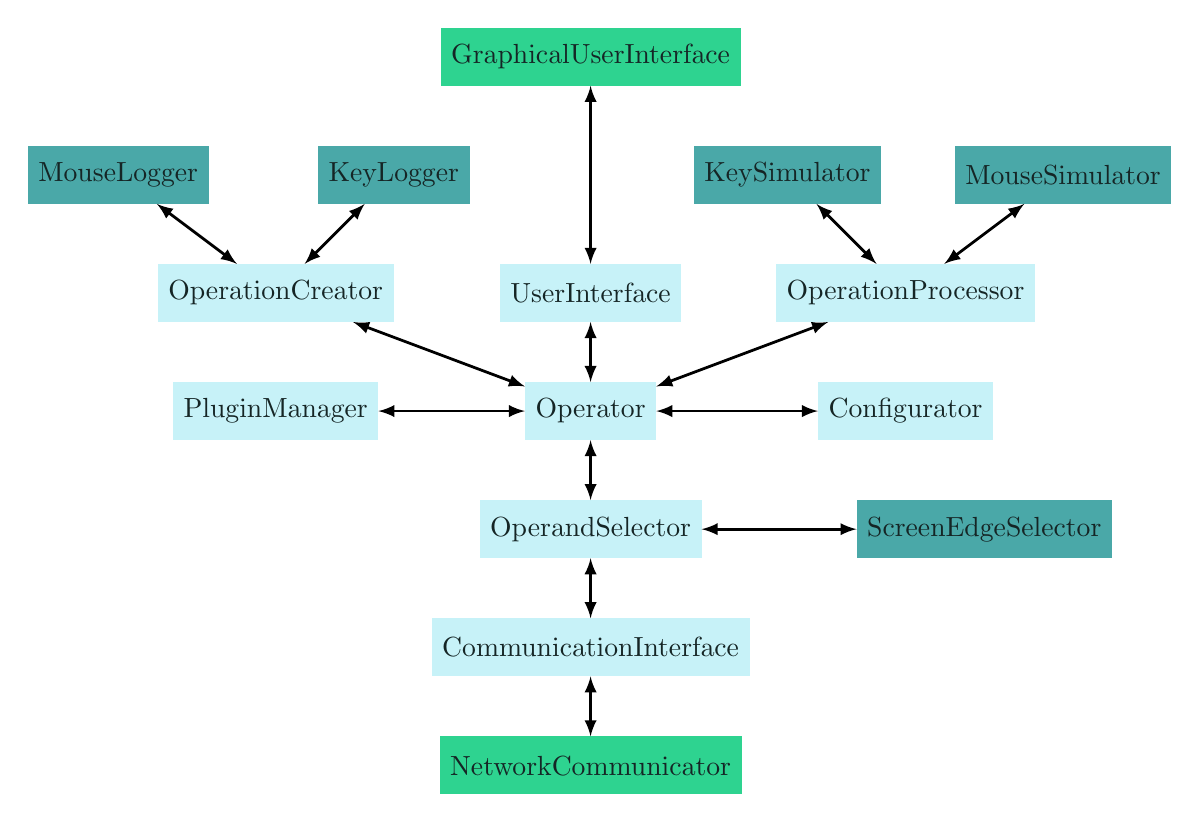
\begin{tikzpicture}
\node[gn] (gui) at (6, 3) {\nodegui};
\node[bn] (ui) at (6, 0) {\nodeui};
\node[bn] (pm) at (2, -1.5) {\nodepm};
\node[bn] (conf) at (10, -1.5) {\nodeconf};
\node[bn] (o) at (6, -1.5) {\nodeo};
\node[bn] (oc) at (2, 0) {\nodeoc};
\node[bn] (op) at (10, 0) {\nodeop};
\node[bn] (os) at (6, -3) {\nodeos};
\node[bn] (ci) at (6, -4.5) {\nodeci};
\node[gn] (nm) at (6, -6) {\nodenm};
\node[dn] (ml) at (0, 1.5) {\nodeml};
\node[dn] (kl) at (3.5, 1.5) {\nodekl};
\node[dn] (ms) at (12, 1.5) {\nodems};
\node[dn] (ks) at (8.5, 1.5) {\nodeks};
\node[dn] (ses) at (11, -3) {\nodeses};
\draw [<->] (gui) -- (ui);
\draw [<->] (ui) -- (o);
\draw [<->] (pm) -- (o);
\draw [<->] (o) -- (conf);
\draw [<->] (oc) -- (o);
\draw [<->] (o) -- (op);
\draw [<->] (kl) -- (oc);
\draw [<->] (ml) -- (oc);
\draw [<->] (op) -- (ks);
\draw [<->] (op) -- (ms);
\draw [<->] (o) -- (os);
\draw [<->] (os) -- (ci);
\draw [<->] (ci) -- (nm);
\draw [<->] (os) -- (ses);
\end{tikzpicture}
\captionof{figure}{Schéma architektury}
\end{center}

\subsubsection{Rozdělení softwarových komponent}
\paragraph{Jádro}
tvoří všechny světle modré komponenty. Bude naprogramováno jako univerzální, tudíž mu bude stačit dodat nějaké uživatelské a komunikační rozhraní a celý program bude fungovat. To znamená, že když někdo sestrojí a naprogramuje mechanické uživatelské rozhraní a komunikační rozhraní pracující s kouřovými signály, bude moct provádět s těmito rozhraními kompatibilní operace.

\paragraph{Komponenty z pluginů}
jsou komponenty mající tmavě modrou barvu. Tvoří samotnou realizaci operací. Operace, které budou konfigurovatelné, budou závislé na použitém uživatelském rozhraní. Nebudou-li operace implementovat podporu pro použité uživatelské rozhraní, bude možné provádět jejich konfiguraci pouze editací konfiguračního souboru. Dále také bude nutné použít vhodné komunikační rozhraní (implementaci CommunicationInterfaceu) pro zajištění fungování všech požadovaných operací, například sdílení myši na systému komunikace pomocí kouřových signálů způsobí nepohodlné používání této operace. Operace mohou být dále závislé na použitém operačním systému.

\paragraph{Implementace komunikačních rozhraní}
jsou znázorněny zelenou barvou. Grafické uživatelské rozhraní slouží k zajištění komunikace mezi uživatelem a programem a NetworkCommunicator bude sloužit k zajištění komunikace mezi navzájem komunikujícími systémy (počítači).

\paragraph{O (ne)závislosti NetworkOperatoru} 
Použité implementace komunikačních rozhraní způsobí natolik zásadní závislost na vlastnostech systému, na kterém je NetworkOperator spuštěn, že pokud je daný systém nekompatibilní, pak se program buď nespustí nebo je po spuštění ukončen chybou.\\
Použité pluginy způsobí také závislost na vlastnostech systému, na němž je jejich fungování požadováno, ovšem v případě jejich nekompatibility není NetworkOperator ukončen, ale pouze nebude možné nekompatibilní operace používat.

\subsubsection{Softwarové komponenty jádra}
\paragraph{\nodeo}
Přijímá požadavky svých sousedů, zpracovává je a předává dál. Tato komponenta také bude spravovat vlákna jádra a řídit proces načítání. Dále bude Operator obsahovat tabulku (identifikátorů) operací a jejich stavů. Při každé změně této tabulky bude o této změně informována každá komponenta, která se zaregistruje do seznamu informovaných komponent pro tuto tabulku. Tento seznam bude také součástí Operatoru. Stav operací bude měněn převážně přes uživatelské rozhraní, jelikož jeden z hlavních významů existence seznamu operací a jejich stavů je umožnit uživateli operace pozastavit a znovu spustit.\\\\
\textbf{\textit{Hlavní problémy k řešení:}} správné předávání informací, registr operací, řízení vláken a načítání programu

\paragraph{\nodepm}
Bude načítat pluginy obsahující definice operací z předem smluveného adresáře na disku. PluginManager projde všechny *.dll soubory v tomto adresáři a pokusí se je načíst jako pluginy. K tomuto účelu bude používat reflection. V případě, že některý ze souborů nebude validní plugin, předá PluginManager tuto informaci Operatoru, který ji předá UserInterfaceu a to zpracuje tuto zprávu (předá ji uživateli).\\\\
\textbf{\textit{Hlavní problém k řešení:}} načítání pluginů pomocí reflection

\paragraph{\nodeconf} 
Zajišťuje uložení a načtení konfigurace.\\\\
Konfigurovatelná třída bude třída implementující rozhraní IConfigurable, které vznikne právě za tímto účelem. Tím se zaváže ke schopnosti zpracovávat TextReader.\\\\
Konfigurační soubor bude textový soubor obsahující všechny konfigurační informace všech konfigurovatelných tříd NetworkOperatoru. Bude rozdělen na oddíly, kdy každý oddíl bude identifikován názvem konfigurovatelné třídy, které daný oddíl patří.\\\\
Načtení konfigurace bude fungovat tak, že Configurator obdrží konfigurovatelný objekt a předá mu TextReader, ze kterého si bude moct přečíst patřičný oddíl konfiguračního souboru.\\\\\
Configurator bude umět také na požádání uložit konfiguraci jakékoliv konfigurovatelné třídy.\\\\
\textbf{\textit{Hlavní problém k řešení:}} práce s textovými soubory.

\paragraph{\nodeoc} 
přijímá požadavky na provedení operací, převádí je na operace a ty předává ke zpracování Operatoru. Zásadní pro OperationCreator bude způsob, jakým tyto požadavky bude přijímat a zpracovávat. OperationCreator totiž bude sloužit jako rozhraní pro komunikaci mezi operacemi a Operatorem a všechny operace do něj budou muset zaregistrovat svůj OperationRequestCreator. Ve chvíli, kdy nějaký OperationRequestCreator OperatorCreatoru předá požadavek na vytvoření operace, zařadí daný požadavek do fronty uvnitř OperationCreatoru. Vzhledem k tomu, že každý OperationRequestCreator bude pracovat na vlastním vlákně, bude zde více vláken sdílet jednu frontu. Z tohoto důvodu bude tato fronta lock-free, čímž se zajistí synchronizace a bezpečné vytváření požadavků na vytvoření operací. OperationCreator schválí každý požadavek na vytvoření operace, která má v Operatoru nastaven stav "runnning" nebo "ready" tím, že jej převede na operaci, což provede tím způsobem, že k datům z požadavku přidá identifikátor operace, které zjistí od Operatoru dle informací z požadavku na vytvoření operace. Pokud se nachází v jiném stavu, je požadavek na vytvoření operace zamítnut a vymazán. OperationCreator bude zaregistrován v seznamu informovaných komponent pro tabulku operací a jejich stavů a ve chvíli, kdy se změní stav některé operace, informuje o této skutečnosti nejen Operator OperationCreatora, ale i OperationCreator příslušný OperationRequestCreator. Tímto způsobem bude možné běžící operace pozastavovat a pozastavené opět spouštět nebo rušit běžící nebo pozastavené operace.\\\\
\textbf{\textit{Hlavní problémy k řešení:}} registry OperationRequestCreatorů, převádění (platných) \\požadavků na operaci na operace, lock-free fronta, pozastavování / spouštění operací

\paragraph{\nodeop}
Bude sloužit jako rozhraní pro komunikaci mezi operacemi a Operatorem a každá operace do něj zaregistruje svůj ActionRequestProcessor, kterému je poté přiřazeno vlákno, tudíž každý ActionRequestProcessor poběží na samostatném vlákně. OperationProcessor bude mít tabulku front, kde každá fronta bude patřit jednomu ActionRequestProcessoru. Bude totiž přijímat operace od Operatoru a převádět je na požadavky na akci, které umístí příslušnému ActionRequestProcessoru do jeho fronty. Každý ActionRequestProcessor pak provádí akce dle požadavků ze své fronty. Stejně jako u OperationCreatoru, bude zde třeba použít lock-free frontu, protože vlákno, které bude naplňovat fronty ActionRequestPorcesorů, bude jiné než každé z vláken, která požadavky z fronty vybírají. OperationProcessor bude zaregistrován v seznamu informovaných komponent pro tabulku operací a jejich stavů a ve chvíli, kdy se změní stav některé operace, informuje o této skutečnosti nejen Operator OperationProcessor, ale i OperationProcessor příslušný ActionRequestProcessor. Tímto způsobem bude možné běžící operace pozastavovat a pozastavené opět spouštět nebo rušit běžící nebo pozastavené operace.\\\\
\textbf{\textit{Hlavní problémy k řešení:}} registr ActionRequestProcessorů a lock-free front, převádění operací na požadavky na akci a předávání požadavků na akci, pozastavování / spouštění operací

\paragraph{\nodeos} 
Přijímá operace k odeslání od Operatoru a zajišťuje výběr cílových počítačů, na kterých se má operace provést. K operaci přidá jméno komunikanta, kterému se má daná operace poslat. K tomu bude mít pro každou operaci zaregistrovaný její vlastní OperandSelector, který bude obsahovat popis způsobu, jakým se operandy vybírají a informaci o tom, zdali je konfigurovatelný a pokud ano, tak implementace různých způsobů, jak jej konfigurovat (například formuláře včlenitelné do GUI apod.). Existence adresáta bude ověřena u komunikačního rozhraní. Operace s přidaným jménem komunikanta pak putuje do CommunicationInterfaceu.\\ OperandSelectory různých počítačů si spolu budou moct vyměňovat zprávy. Zprávy, které si mezi sebou budou vyměňovat OperandSelectory různých počítačů, se již dále jádrem NetworkOperatoru (směrem k Operatoru) nebudou šířit.\\\\
\textbf{\textit{Hlavní problémy k řešení:}} registr OperandSelectorů, přidávání adresátů k operacím, vzájemná komunikace OperandSelectorů

\paragraph{\nodeci}
Bude sloužit jako komunikační rozhraní mezi jádrem NetworkOperatoru a nějakou konkrétní realizací komunikátoru. Bude jádru (konkrétně OperandSelectoru) předávat přijaté zprávy a operace a zprostředkovávat odeslání zpráv dalším komunikantům.\\\\
\textbf{\textit{Hlavní problém k řešení:}} komunikace mezi jádrem NetworkOperatoru a nějakou konkrétní realizací komunikátoru

\paragraph{\nodeui}
Bude sloužit jako komunikační rozhraní mezi jádrem NetworkOperatoru a nějakou konkrétní realizací uživatelského rozhraní. Bude jádru (konkrétně Operatoru) předávat požadavky uživatele a realizaci uživatelského rozhraní zprávy z jádra NetworkOperatoru.\\\\
\textbf{\textit{Hlavní problém k řešení:}} komunikace mezi jádrem NetworkOperatoru a nějakou konkrétní realizací uživatelského rozhraní

\subsubsection{Softwarové komponenty pluginů}
\paragraph{\nodekl} 
Bude implementací OperationRequestCreatoru pro operaci sdílení klávesnice, bude monitorovat klávesnici a převádět všechny vstupy uživatele pomocí klávesnice na požadavky na operaci. To bude zajištěno tím, že KeyLogger bude pracovat s knihovnou pro monitorování a simulování klávesnice, která bude napsána v C++ a která bude komunikovat s Windows API, od kterého se dozví, jaké vstupy uživatel klávesnicí provedl. Popis vstupu bude předán z C++ knihovny do v C\#u napsané části KeyLoggeru, která se postará o vytvoření požadavku na vznik operace a jeho předání OperationCreatoru.\\\\
\textbf{\textit{Hlavní problém k řešení:}} spolupráce C\#u a C++

\paragraph{\nodeml} 
Bude fungovat analogicky jako KeyLogger, pouze s tím rozdílem, že bude pracovat s daty popisujícími vstupy myši pomocí k tomuto účelu napsané C++ové knihovny.\\\\
\textbf{\textit{Hlavní problém k řešení:}} spolupráce C\#u a C++

\paragraph{\nodeks} 
Bude provádět akce uživatelského vstupu pomocí klávesnice. De facto půjde o simulátor klávesnice. To bude zajištěno tím, že KeySimulator bude pracovat s knihovnou pro monitorování a simulování klávesnice, která bude napsána v C++ a která bude komunikovat s Windows API. Tato knihovna bude používána C\#ovým kódem.\\\\
\textbf{\textit{Hlavní problém k řešení:}} spolupráce C\#u a C++

\paragraph{\nodems} 
Bude fungovat analogicky jako KeySimulator, pouze s tím rozdílem, že bude provádět akce myši pomocí k tomuto účelu napsané C++ové knihovny.\\\\
\textbf{\textit{Hlavní problém k řešení:}} spolupráce C\#u a C++

\paragraph{\nodeses}
Bude jediný implementovaný OperandSelector. Bude si vždy pamatovat jednoho adresáta a bude komunikovat s MouseSimulatorem a MouseLoggerem, od kterých bude zjišťovat, zdali se kurzor myši nenachází na okraji (hraně) monitoru. Pokud ano, tak dle uživatelské konfigurace (kterou dostane od Configuratoru a která bude obsahovat matici sousednosti jednotlivých adresátů) změní adresáta na zařízení, které je se zařízením sousední přes danou hranu (viz uživatelská specifikace). Není-li toto zařízení dostupné (například není připojené k síti), vybere dalšího adresáta ve stejném směru. Pokud neexistuje daný soused (například se adresát bude nacházet na okraji matice sousednosti adresátů), adresát se nemění. Ve výchozím stavu je operandem počítač, jehož myš je myší sdílenou. Pokud bude adresát počítač, jehož myš se sdílí, pak se operace neposílají. Ve chvíli, kdy MouseSimulator změní polohu myši nebo MouseLogger detekuje její pohyb, informují tyto komponenty ScreenEdgeSelector daného komunikanta, který je buď tím, jehož myš se sdílí, pak se informace o změně polohy myši zpracuje lokálně, nebo je komunikant zařízením, jehož myš se nesdílí, a pak ScreenEdgeSelector zkontroluje, zdali se myš nenachází na kraji monitoru a pokud ano, pošle komunikantovi, jehož myš se sdílí, zprávu o nutné změně adresáta dalších operací, které ScreenEdgeSelector používají jako OperandSelector.\\\\
EdgeScreenSelector bude též obsahovat WPF komponentu, pomocí které půjde upravovat jeho konfiguraci (matici sousednosti).\\\\
\textbf{\textit{Hlavní problém k řešení:}} správné a včasné střídání adresátů

\subsubsection{Softwarové komponenty sloužící jako implementace komunikačních rozhraní}\paragraph{\nodenm}
Je specifikován v podsekci "Síť".

\paragraph{\nodegui}
Je specifikováno v podsekci "GUI".

\subsubsection{Implementované operace}
V odevzdané verzi budou napsané následující operace:

\paragraph{Sdílení myši}
\begin{enumerate}[leftmargin=5mm]
\item OperationRequestCreator této operace bude MouseLogger.
\item ActionRequestProcessor této operace bude MouseSimulator.
\item OperandSelector této operace bude EdgeOperandSelector.
\item Tato operace nebude konfigurovatelná.
\end{enumerate}

\paragraph{Sdílení klávesnice}
\begin{enumerate}[leftmargin=5mm]
\item OperationRequestCreator této operace bude KeyLogger.
\item ActionRequestProcessor této operace bude KeySimulator.
\item OperandSelector této operace bude EdgeOperandSelector.
\item Tato operace nebude konfigurovatelná.
\end{enumerate}

\subsubsection{Ukázka provedení operace}
\paragraph{Znázornění povedení operace}
je graf, který splňuje následující:
\begin{enumerate}[leftmargin=5mm]
\item Znázornění provedení operace je schéma architektury.
\item Tmavě zelené komponenty jsou ty, které se budou podílet na provedení dané operace, světle modré ty ostatní.
\end{enumerate}

\paragraph{Vytvoření operace stisknutí klávesy na zdrojovém počítači}
Nechť je počítač, který vytvoří operaci, nazýván zdrojový. Pak je vytvoření operace stisknutí klávesy na zdrojovém počítači následující posloupnost kroků:
\begin{enumerate}[leftmargin=5mm]
\item Uživatel stiskne klávesu na zdrojovém počítači.
\item Informace o stisku klávesy se šíří do OS, kde je dostupná přes Windows API.
\item KeyLogger se o stisku klávesy dozvídá od Windows API a vytváří požadavek na vytvoření operace. 
\item Dokud OperationCreator nemá žádné OperationRequesty, pasivně čeká. Jakmile však nějaký dostane, tak pokud není operace pozastavena, vytvoří ji a předá Operatoru.
\item Operator předá operaci OperandSelectoru.
\item OperandSelector zjistí adresáta přes EdgeScreenSelector, tuto informaci k operaci přidává a odevzdává operaci komunikačnímu rozhraní k odeslání.
\item ComunicationInterface předává operaci NetworkComunicatoru k odeslání.
\item NetworkCommunicator odešle operaci adresátovi. 
\end{enumerate}
Komponenty, které byly použity pro vytvoření operace stisknutí klávesy na zdrojovém počítači, lze vidět na následujícím znázornění povedení operace:

\begin{center}
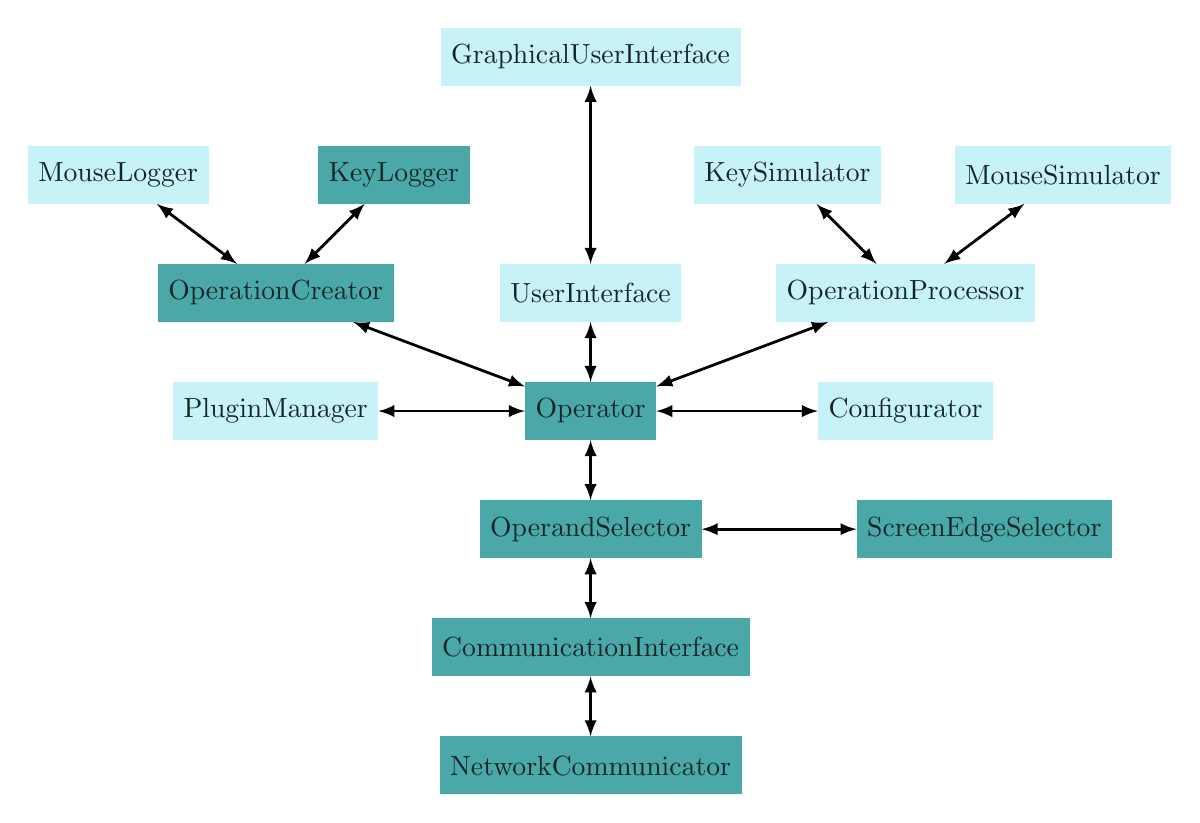
\begin{tikzpicture}
\node[bn] (gui) at (6, 3) {\nodegui};
\node[bn] (ui) at (6, 0) {\nodeui};
\node[bn] (pm) at (2, -1.5) {\nodepm};
\node[bn] (conf) at (10, -1.5) {\nodeconf};
\node[dn] (o) at (6, -1.5) {\nodeo};
\node[dn] (oc) at (2, 0) {\nodeoc};
\node[bn] (op) at (10, 0) {\nodeop};
\node[dn] (os) at (6, -3) {\nodeos};
\node[dn] (ci) at (6, -4.5) {\nodeci};
\node[dn] (nm) at (6, -6) {\nodenm};
\node[bn] (ml) at (0, 1.5) {\nodeml};
\node[dn] (kl) at (3.5, 1.5) {\nodekl};
\node[bn] (ms) at (12, 1.5) {\nodems};
\node[bn] (ks) at (8.5, 1.5) {\nodeks};
\node[dn] (ses) at (11, -3) {\nodeses};
\draw [<->] (gui) -- (ui);
\draw [<->] (ui) -- (o);
\draw [<->] (pm) -- (o);
\draw [<->] (o) -- (conf);
\draw [<->] (oc) -- (o);
\draw [<->] (o) -- (op);
\draw [<->] (kl) -- (oc);
\draw [<->] (ml) -- (oc);
\draw [<->] (op) -- (ks);
\draw [<->] (op) -- (ms);
\draw [<->] (o) -- (os);
\draw [<->] (os) -- (ci);
\draw [<->] (ci) -- (nm);
\draw [<->] (os) -- (ses);
\end{tikzpicture}
\captionof{figure}{Vytvoření operace na zdrojovém počítači}
\end{center}

\paragraph{Provedení operace stisknutí klávesy na cílovém počítači}
Nechť je počítač, na kterém je operace prováděna označen jako cílový. Pak je provedení operace stisknutí klavesy na cílovém počítači následující posloupnost kroků:
\begin{enumerate}[leftmargin=5mm]
\item NetworkCommunicator přijímá operaci, která se postupně předá CommunicationInterfacu, OperandSelectoru (i EdgeScreenSelectoru) a skončí u Operatora.
\item Operator předá operaci OperationProcessoru.
\item OperationProcessor z operace vytvoří ActionRequest, který zařadí do fronty příslušnému ActionRequestPorcessoru.
\item Každý ActionRequestProcessor pasivně čeká, než dostane nějaký ActionRequest do své fronty. Jakmile nějaký přijde, ActionRequestProcessor se probouzí a provádí požadovanou akci.
\end{enumerate}
Komponenty, které byly použity pro provedení operace stisknutí klávesy na cílovém počítači, lze vidět na následujícím znázornění povedení operace:

\begin{center}
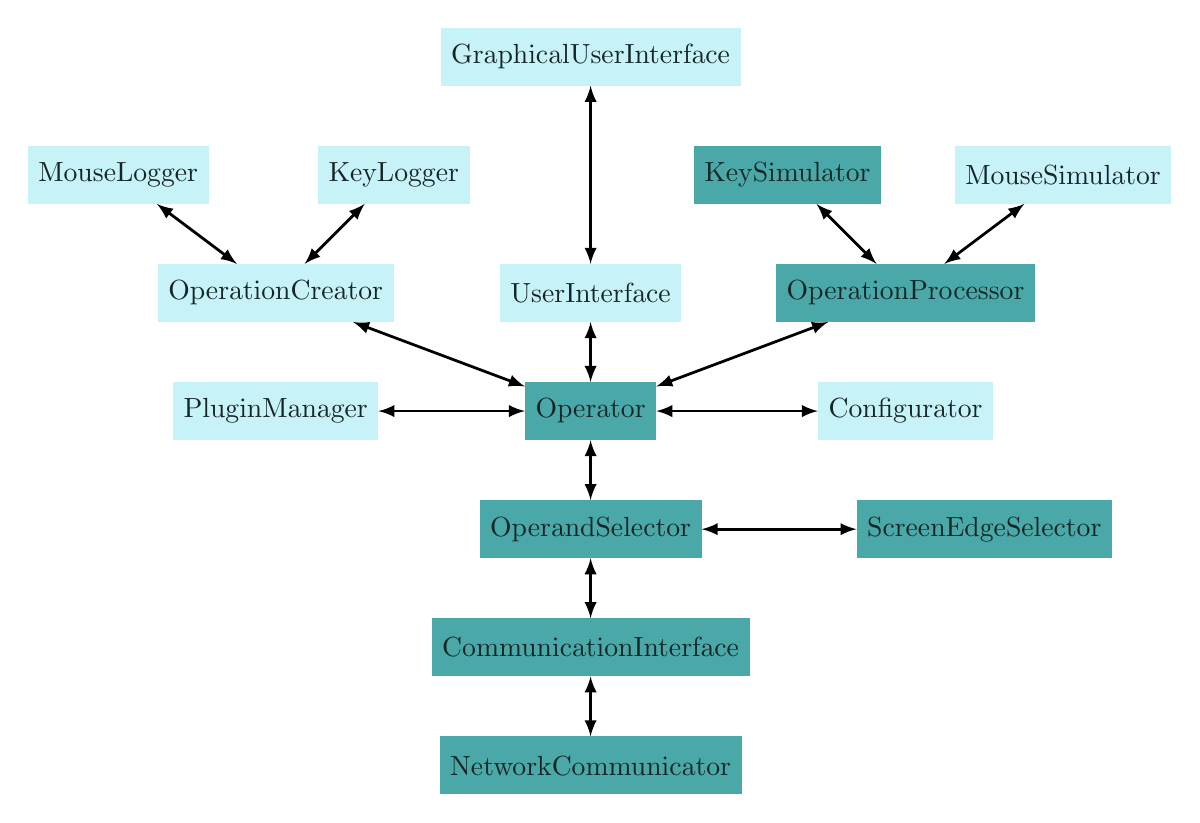
\begin{tikzpicture}
\node[bn] (gui) at (6, 3) {\nodegui};
\node[bn] (ui) at (6, 0) {\nodeui};
\node[bn] (pm) at (2, -1.5) {\nodepm};
\node[bn] (conf) at (10, -1.5) {\nodeconf};
\node[dn] (o) at (6, -1.5) {\nodeo};
\node[bn] (oc) at (2, 0) {\nodeoc};
\node[dn] (op) at (10, 0) {\nodeop};
\node[dn] (os) at (6, -3) {\nodeos};
\node[dn] (ci) at (6, -4.5) {\nodeci};
\node[dn] (nm) at (6, -6) {\nodenm};
\node[bn] (ml) at (0, 1.5) {\nodeml};
\node[bn] (kl) at (3.5, 1.5) {\nodekl};
\node[bn] (ms) at (12, 1.5) {\nodems};
\node[dn] (ks) at (8.5, 1.5) {\nodeks};
\node[dn] (ses) at (11, -3) {\nodeses};
\draw [<->] (gui) -- (ui);
\draw [<->] (ui) -- (o);
\draw [<->] (pm) -- (o);
\draw [<->] (o) -- (conf);
\draw [<->] (oc) -- (o);
\draw [<->] (o) -- (op);
\draw [<->] (kl) -- (oc);
\draw [<->] (ml) -- (oc);
\draw [<->] (op) -- (ks);
\draw [<->] (op) -- (ms);
\draw [<->] (o) -- (os);
\draw [<->] (os) -- (ci);
\draw [<->] (ci) -- (nm);
\draw [<->] (os) -- (ses);
\end{tikzpicture}
\captionof{figure}{Provedení operace na cílovém počítači}
\end{center}

\subsection{Síť}
V této sekci je popsáno, jakým způsobem bude fungovat vzájemné propojení počítačů, které budou připojeny k jedné počítačové síti (broadcast doméně) a bude na nich běžet NetworkOperator.
\subsubsection{Topologie propojení}
Topologie vzájemného propojení počítačů (abstraktně, nad počítačovou sítí) bude hvězdicová, kdy centrální prvek bude nazýván "server" a všechny počítače k němu budou připojeny. Každý k serveru připojený počítač budeme nazývat "klient". Server bude také klient. Klientům a serveru budeme interně říkat "síť", tudíž když mluvím o síti, ignoruji tím ty počítače, na kterých neběží NetworkOperator.

\subsubsection{Operace NetworkCommunicatoru}
Operace NetworkCommunicatoru budou následující:
\begin{enumerate}
\item Vytvoření sítě
\item Připojení k síti
\item Odpojení od sítě
\item Odeslání operace jinému zařízení v síti
\item Přijetí operace od jiného zařízení v síti
\item Zkontrolování stavu jakéhokoliv počítače, který je připojený k síti.
\end{enumerate}

\paragraph{Vytvoření sítě} 
Bude fungovat tak, že všechna zařízení, která budou chtít vytvořit síť, začnou broadcastovat informaci o svém potenciálu být server. Tento potenciál bude číslo mající následující hodnotu:
$$((\sum_{p \in \{procesory\ klienta\}} frekvence(p) * 100) + l) * r ,$$ 
kde $l$ je rychlost linky v Mbit/s, kterou je počítač připojený k síti, $r$ je velikost operační paměti klienta v GB a $frekvence$ je zobrazení z množiny procesorů do $R$, kde $\forall f \in rng(frekvence)$ je frekvence procesoru v GHz.\\\\
Každý počítač si bude zachytávat broadcastované zprávy všech ostatních počítačů a přidávat je do tabulky všech počítačů v síti, kde si bude pro každý počítač pamatovat jeho adresu a potenciál být serverem. Do této tabulky zahrne každý počítač i sám sebe. Ve chvíli, kdy mají všechny počítače tuto tabulku kompletní, vybere se mezi nimi server. Serverem se stane ten z počítačů s nejvyšším potenciálem být serverem, jeho adresa v síti bude nejnižší. Server determinuje, že se má stát serverem a začne se jako server chovat, tudíž bude přijímat požadavky od ostatních zařízení na připojení do sítě, což bude právě to, co ostatní počítače udělají. Všichni klienti také se také zbaví všech informací o ostatních klientech, budou tedy znát jen adresu serveru. Server si od každého připojeného klienta vyžádá jméno, které automaticky pošle všem klientům v síti. Klienti si budou pamatovat jména ostatních klientů a používat je jako identifikátory příjemců operací (adresátů). Adresy klientů zná pouze server. Ve chvíli, kdy se připojí k právě vytvořenému serveru poslední klient, který se podílel na vytváření sítě, je síť vytvořena.

\paragraph{Připojení k síti} 
Když se chce klient připojit k síti, tak pokud zná adresu serveru, připojí se k němu bez problému způsobem popsaným výše. Pokud klient adresu nezná, začne vysílat broadcast zprávu obsahující jeho potenciál být serverem do broadcast domény, kde pokud žádný server neposlouchá, tak se vytvoří síť a pokračuje se způsobem popsaným výše. Pokud již síť byla vytvořena a existuje v ní server, který dostane broadcast zprávu, pošle klientovi informace, pomocí kterých se k serveru připojí stejným způsobem, jako se připojí klienti vytvářející síť.

\paragraph{Odpojení od sítě} 
Klient serveru oznámí, že se odpojuje od sítě a server o této skutečnosti informuje všechny ostatní klienty. S probíhajícími operacemi se vypořádá každý klient podle vůle uživatele. Pokud se od sítě odpojí server, oznámí  tuto skutečnost klientům a ti vytvoří síť znovu s jiným serverem.

\paragraph{Odeslání operace jinému zařízení v síti} 
Bude fungovat tak, že klient pošle operaci se jménem příjemce serveru a server ji odešle příjemci.

\paragraph{Přijetí operace od jiného zařízení v síti} 
Operace bude přijata od serveru, kterému ji nějaké jiné zařízení poslalo předtím.

\paragraph{Kontrola stavu jiného klienta} 
Bude moct být na požádání provedena serverem. Server bude tuto kontrolu provádět pravidelně sám.

\paragraph{Vlákna v NetworkCommunicatoru}
Klient bude používat jedno vlákno, server bude používat jedno vlákno pro každého připojeného klienta a jedno hlavní vlákno.

\paragraph{Poznámka} 
Součásti server a klient budou obsaženy v NetworkCommunicatoru.

\subsection{Grafické uživatelské rozhraní}
Bude napsáno ve WPF. Na následujících stránkách je popsán návrh grafického uživatelského rozhraní (návrh se může od výsledku vzhledově drobně lišit). GUI bude komunikovat s jádrem NetworkOperatoru přes komponentu UserInterface. Tuto komunikaci blíže specifikovat nebudu, myslím, že je jasné, jaké z informací z GUI jsou založeny na informacích získaných od jádra NetworkOperatoru. GUI poběží na vlastním vlákně (viz "Proces spouštění").

\subsubsection{Načítací obrazovka}
\begin{figure}[H]
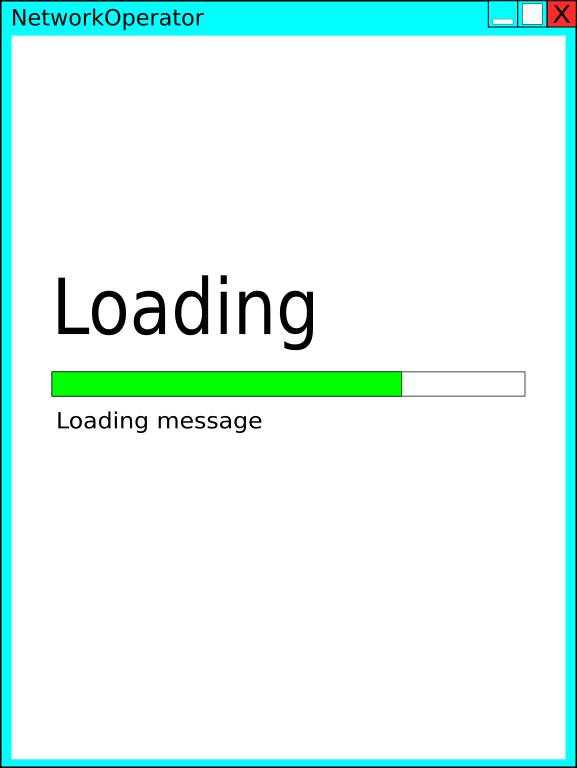
\includegraphics[width=8cm]{gui1-loading.png}
\centering
\end{figure}

Po spuštění se zobrazí načítací obrazovka, která bude zobrazovat informace o průběhu načítání pluginů a procesu vytváření sítě. Zprávy "Loading" a "Loading message" budou do GUI předávány z jádra NetworkOperatoru a budou se v průběhu načítání měnit dle situace. Po dokončení spuštění NetworkOperatoru a sítě se zobrazí ovládací panel. 

\subsubsection{Ovládací panel}
\begin{figure}[H]
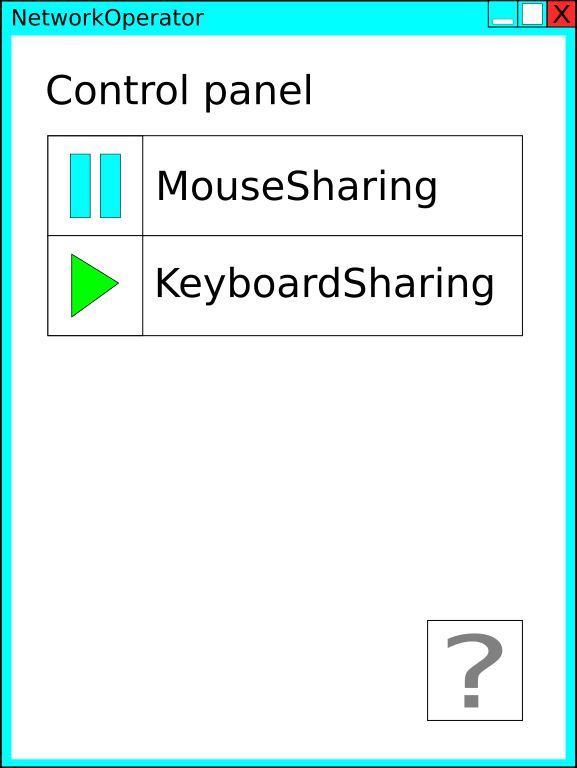
\includegraphics[width=8cm]{gui2-control-panel.png}
\centering
\end{figure}

Bude obsahovat tabulku všech dostupných operací, která bude mít dva sloupce. V prvním sloupci bude tlačítko pro změnu stavu obsahující ikonu reprezentující výsledný stav operace po provedení dané změny. Běžící operace tedy půjde pozastavovat a pozastavené operace spouštět.\\\\
Ve druhém sloupci bude název operace. Pokud na něj uživatel klikne, zobrazí se přehled dané operace.\\\\
Tato tabulka bude napsána jako vlastní WPF ovládací prvek (WPF Control).\\\\
Dále zde bude tlačítko s otazníkem, na které když uživatel klikne, otevře se uživatelská dokumentace NetworkOperatoru ve výchozím webovém prohlížeči uživatele.

\subsubsection{Přehled běžící operace}
\begin{figure}[H]
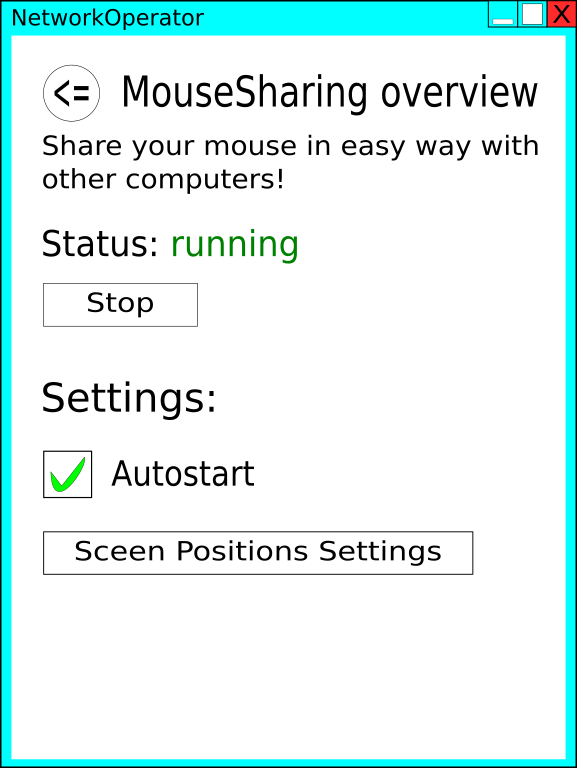
\includegraphics[width=8cm]{gui3-mousesahring-overview-running.png}
\centering
\end{figure}

Předpokládejme, že uživatel v ovládacím panelu klikne na "MouseSharing". Poté se mu zobrazí přehled výše. V přehledu bude název operace, krátký popis operace, ukazatel stavu operace, tlačítko umožňující změnu stavu operace a nastavení.\\\\
Pokud by operace měla nějaké vlastní nastavení (obsažené v pluginu, který musí podporovat konfiguraci přes WPF), zobrazilo by se bezprostředně po nadpisu "Settings".\\\\
Dále zde bude zaškrtávací box s nápisem "Autostart", kterým půjde upravovat, zdali se daná operace (její provádění) spustí po načtení NetworkOperatoru. Tato konfigurace bude nezávislá na jádře NetworkOperatoru a jeho Configuratoru, GUI si ho bude zajišťovat samo s tím, že bude řešeno pomocí textového souboru, který bude obsahovat názvy automaticky spouštěných operací.\\\\
Poslední položkou, která tu bude, bude tlačítko "Screen Positions Settings", na které když uživatel klikne, otevře se konfigurace sousednosti monitorů počítačů, kterou bude používat (a WPF prvky k jejímu zajištění dodávat) EdgeScreenSelector.

\paragraph{Tlačítko zpět}
Bude se vždy nacházet vedle nadpisu daného okna a bude vracet GUI o jeden krok zpět, na tu část GUI, ze které se na tu současnou uživatel dostal. Toto tlačítko se vždy bude chovat stejně, proto ho již vícekrát popisovat nebudu.

\subsubsection{Přehled zastavené operace}
\begin{figure}[H]
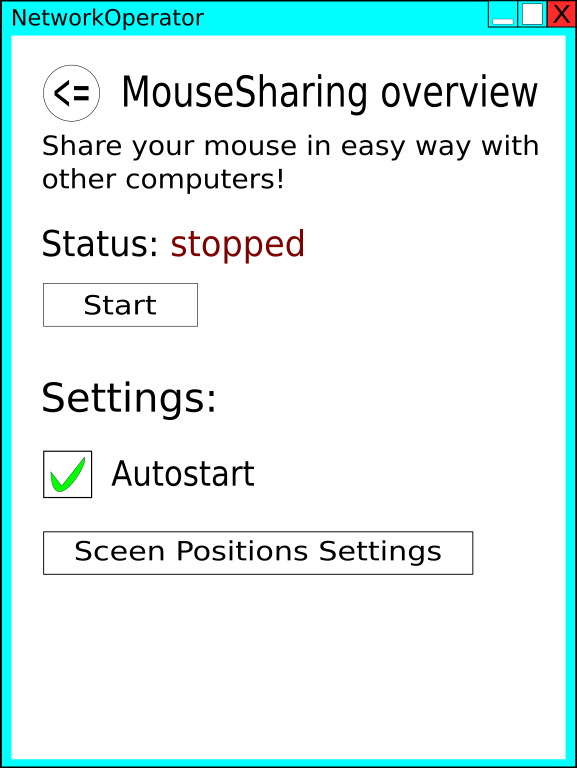
\includegraphics[width=8cm]{gui4-mousesahring-overview-stopped.png}
\centering
\end{figure}

Po zastavení operace kliknutím na tlačítko "Stop" bude vypadat přehled operace jako na obrázku výše.

\paragraph{KeyboardSharing overview}
Bude vypadat analogicky přehledu operace MouseSharing.

\subsubsection{Konfigurace sousednosti monitorů počítačů}
\begin{figure}[H]
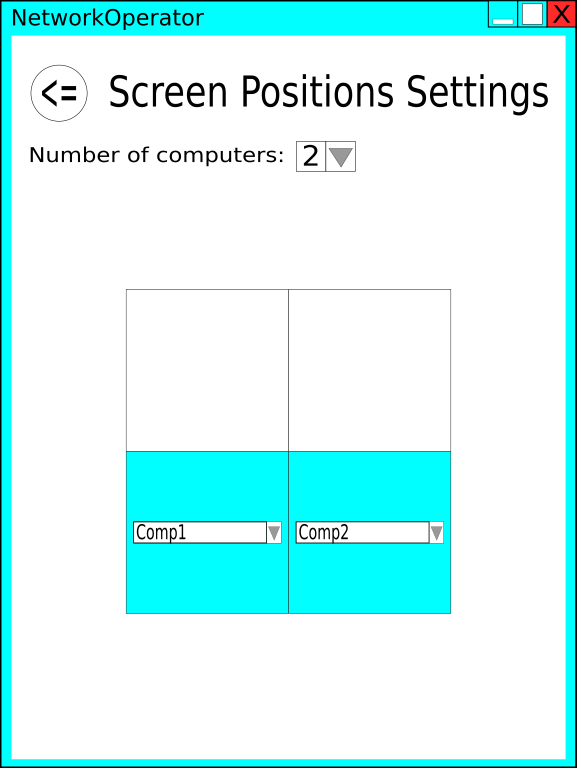
\includegraphics[width=8cm]{gui5-screen-positions-settings.png}
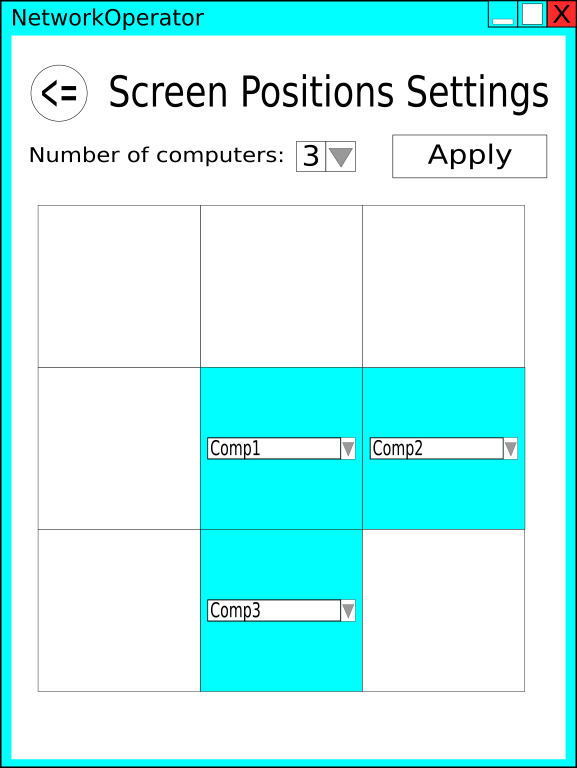
\includegraphics[width=8cm]{gui6-screen-positions-settings-changed.png}
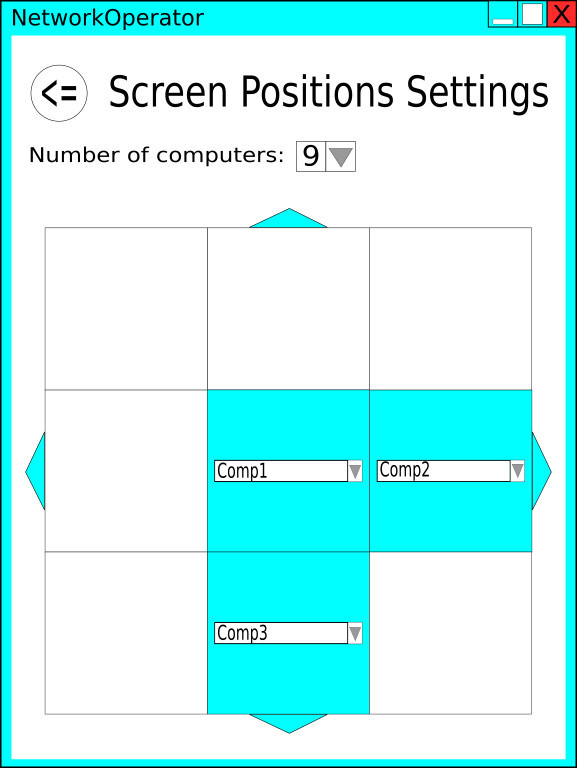
\includegraphics[width=8cm]{gui7-screen-positions-settings-big-matrix.png}
\centering
\end{figure}

Konfigurace sousednosti monitorů počítačů bude obsahovat nadpis, pod kterým se bude nacházet vysouvací seznam s počtem počítačů, pro které chce uživatel nastavit sdílení myši nebo klávesnice (konfigurace obou bude vždy ekvivalentní). Výchozí hodnota bude počet počítačů v síti, pokud nebyla uložena předtím konfigurace, kde bylo nastaveno jiné číslo, nebo počet počítačů uložený v načtené konfiguraci.\\\\
Pod tímto seznamem se bude nacházet samotný konfigurátor matice sousednosti monitorů počítačů.\\\\
Konfigurátor matice sousednosti počítačů bude naprogramovaný pomocí vlastního WPF control, kterému budu říkat BigMatrixLayout.

\paragraph{BigMatrixLayout}
Bude WPF control, který bude obsahovat matici polí, přičemž v každém poli bude moct být jakýkoli WPF control. Ze samotné matice polí uvidí uživatel pouze část (podmatici). Pokud se uživatel bude chtít posunout do oblasti, která není vidět, stačí, aby myší najel nad BigMatrixLayout a s animací se objeví šipky na stranách konfigurace (viz obrázek pro 9 počítačů). Poté bude možné se přesunout do jiné oblasti matice sousednosti kliknutím na nějakou z těchto šipek, přičemž vždy půjde o posun o jednu řadu nebo o jeden sloupec ve směru šipky. Pokud se v nějakém směru nepůjde posunout dál, daná šipka se nezobrazí. Každé pole bude mít nastavitelnou barvu pozadí a bude moct zpracovávat různé události, například kliknutí na něj nebo najetí myší nad něj. Další zásadní vlastností BigMatrixLayoutu bude možnost prohazovat pole. To bude fungovat podobně, jako princip drag\&drop, kdy pro prohození pole bude třeba na pole kliknout levým tlačítkem myši, držet tlačítko stisknuté a pak s polem posouvat hýbáním myší. Pro umístění pole na novou pozici (respektive prohození s polem na nové pozici) bude třeba s polem najet na nové pole a pustit levé tlačítko myši. Při přesouvání nějakého pole bude pole následovat myš a po puštění se s animací dosune na požadované pole z místa, ve kterém se nacházelo, když uživatel pustil levé tlačítko myši (což bude typicky kousek od cílového umístění, takže se samo trochu s animací posune). Pro každé při přesunu překračované pole bude moci programátor rozhodnout, zdali je vhodné nebo ne a podle toho se program zachová. Po puštění levého tlačítka myši na nevhodném poli se operace přesunu pole / prohození polí zruší a přesouvané pole se vrátí na svou původní pozici. Po puštění levého tlačítka myši na vhodném poli se přesun / prohození provede.

\paragraph{Použití BigMatrixLayoutu ke konfiguraci matice sousednosti ScreenEdgeSelectoru}
Nyní popišme, jakým způsobem bude BigMatrixLayout použit (specifikován) ke konfiguraci ScreenEdgeSelectoru. Pole, na kterém bude počítač, bude modré a bude obsahovat vysouvací seznam s názvy dostupných komunikantů a po kliknutí pravým tlačítkem myši na něj se změní v prázdné pole. Pole, které bude prázdné, bude mít stejnou barvu jako pozadí a po kliknutí levým tlačítkem myši na něj se změní na pole obsahující počítač. Při přesunu pole nad nevhodným polem se toto pole zbarví červeně a při přesunu pole nad vhodným polem se toto pole zbarví zeleně.\\\\
Počet počítačů z vysouvacího seznamu pod nadpisem bude upravovat rozměr celé matice, která bude čtvercová. Také bude upravovat maximální počet počítačů, které bude moci uživatel umístit.\\\\
Umísťovat počítače půjde tak, že přidaný / přemístěný počítač musí sdílet nějakou hranu s alespoň jedním umístěným počítačem. První počítač půjde umístit kamkoliv (do prázdné matice).\\\\
BigMatrixLayout bude zabírat až cca 3/4 obsahu okna NetworkOperatoru (viz obrázky výše). Vždy se bude zobrazovat co největší podmatice matice sousednosti ScreenEdgeSelectoru, tak, aby bylo možné pohodlně přečíst data z vysouvacích seznamů. Po změně konfigurace se zobrazí tlačítko Apply (viz 2. obrázek z obrázků výše), po kliknutí na které se nová konfigurace použije pro rekonfiguraci ScreenEdgeSelectoru a uloží se do konfigurace NetworkOperatoru (přes Configurator).

\subsection{Proces spuštění}
\subsubsection{Graf načítání}
Nyní pokročme k popisu spuštění NetworkOperatoru. Tento proces graficky znázorním pomocí posloupnosti grafů načítání, což je graf splňující následující:
\begin{enumerate}[leftmargin=5mm]
\item Graf načítání je schéma architektury.
\item Světle modré vrcholy reprezentují zatím nenačtené komponenty.
\item Zelené vrcholy představují načítané komponenty.
\item Tmavě modré vrcholy jsou aktivní nebo připravené plnit svůj účel, bude-li to třeba.
\end{enumerate}
Nyní již popišme samotný proces spouštění.

\subsubsection{Spuštění programu}
Když je spuštěn program, spustí se na hlavním vlákně GUI. Dále se rozeběhne druhé vlákno, na kterém se spustí jádro NetworkManageru. V GUI se zobrazí načítací obrazovka, která bude postupně uživatele informovat o průběhu načítání dle informací získaných od jádra.
\begin{center}
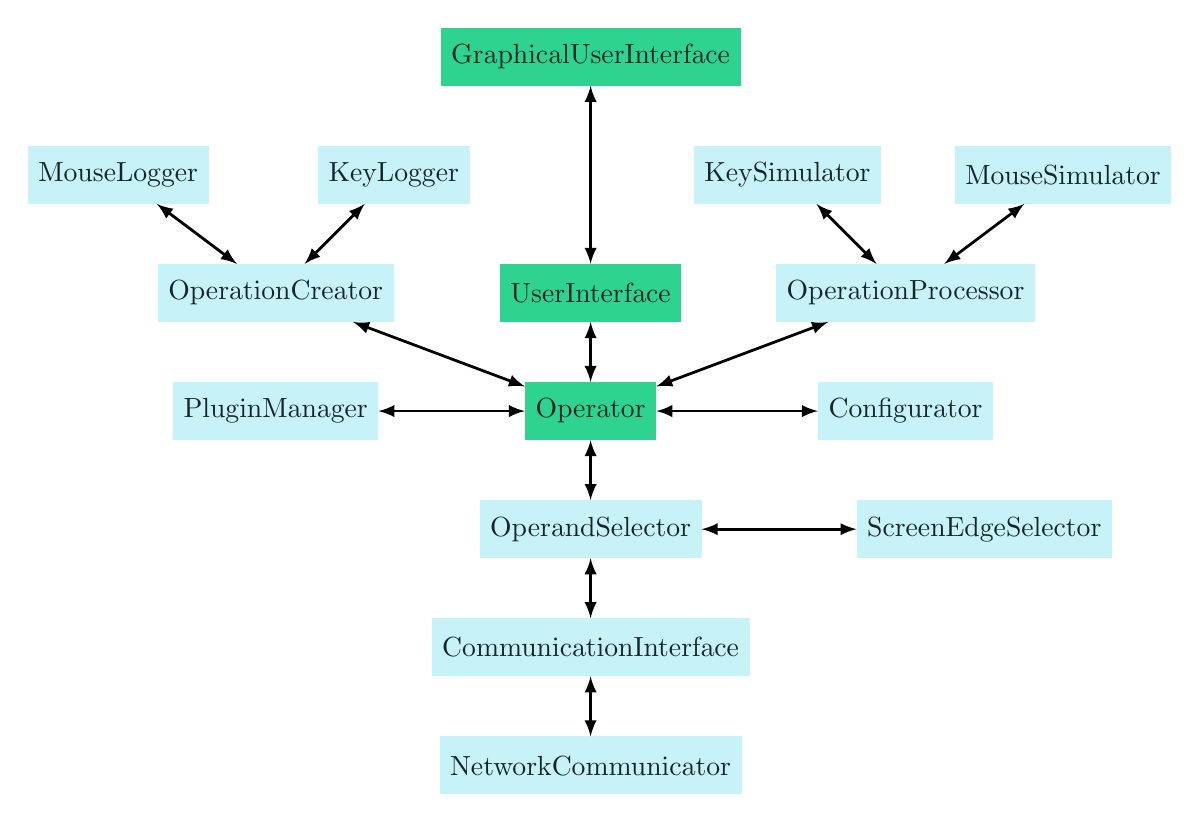
\begin{tikzpicture}
\node[gn] (gui) at (6, 3) {\nodegui};
\node[gn] (ui) at (6, 0) {\nodeui};
\node[bn] (pm) at (2, -1.5) {\nodepm};
\node[bn] (conf) at (10, -1.5) {\nodeconf};
\node[gn] (o) at (6, -1.5) {\nodeo};
\node[bn] (oc) at (2, 0) {\nodeoc};
\node[bn] (op) at (10, 0) {\nodeop};
\node[bn] (os) at (6, -3) {\nodeos};
\node[bn] (ci) at (6, -4.5) {\nodeci};
\node[bn] (nm) at (6, -6) {\nodenm};
\node[bn] (ml) at (0, 1.5) {\nodeml};
\node[bn] (kl) at (3.5, 1.5) {\nodekl};
\node[bn] (ms) at (12, 1.5) {\nodems};
\node[bn] (ks) at (8.5, 1.5) {\nodeks};
\node[bn] (ses) at (11, -3) {\nodeses};
\draw [<->] (gui) -- (ui);
\draw [<->] (ui) -- (o);
\draw [<->] (pm) -- (o);
\draw [<->] (o) -- (conf);
\draw [<->] (oc) -- (o);
\draw [<->] (o) -- (op);
\draw [<->] (kl) -- (oc);
\draw [<->] (ml) -- (oc);
\draw [<->] (op) -- (ks);
\draw [<->] (op) -- (ms);
\draw [<->] (o) -- (os);
\draw [<->] (os) -- (ci);
\draw [<->] (ci) -- (nm);
\draw [<->] (os) -- (ses);
\end{tikzpicture}
\captionof{figure}{Spuštění - spuštění programu}
\end{center}

\subsubsection{Příprava k načtení pluginů}
V této fázi se jádro připraví k procesu načtení OperandSelectorů a operací z pluginů.
\begin{center}
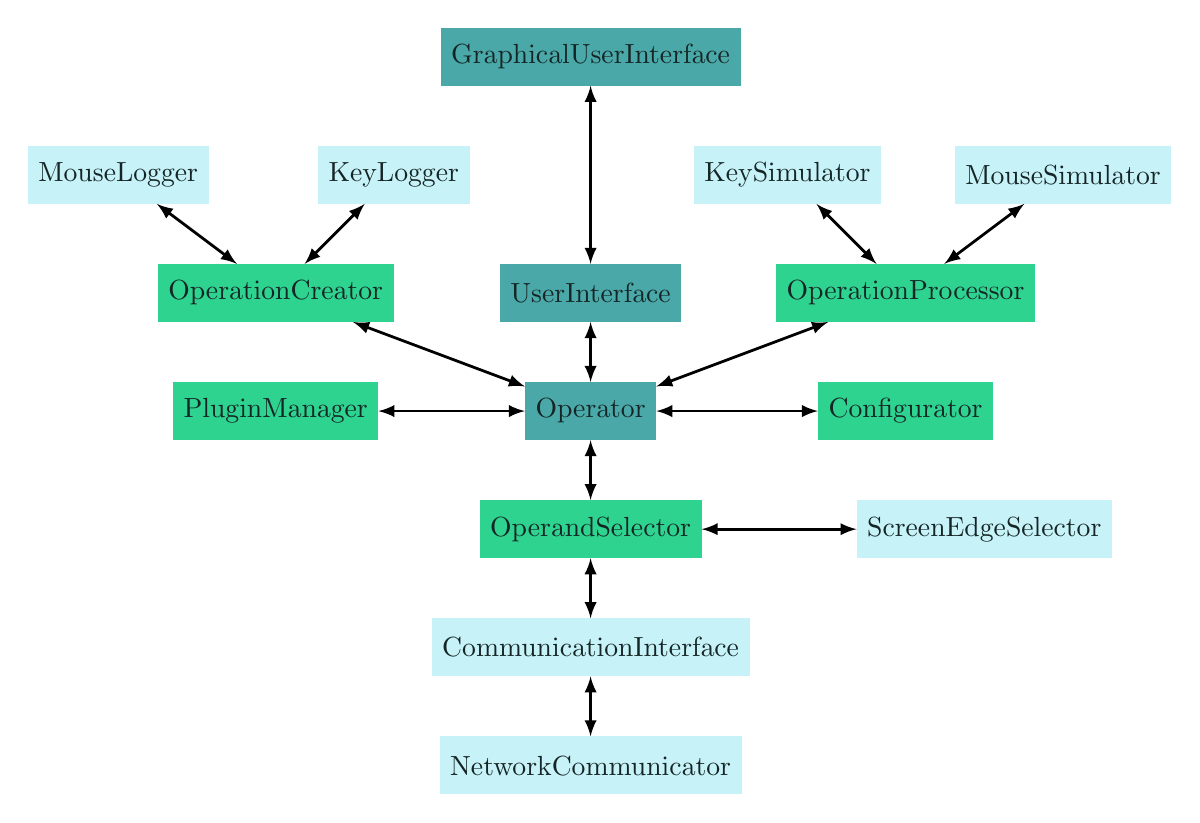
\begin{tikzpicture}
\node[dn] (gui) at (6, 3) {\nodegui};
\node[dn] (ui) at (6, 0) {\nodeui};
\node[gn] (pm) at (2, -1.5) {\nodepm};
\node[gn] (conf) at (10, -1.5) {\nodeconf};
\node[dn] (o) at (6, -1.5) {\nodeo};
\node[gn] (oc) at (2, 0) {\nodeoc};
\node[gn] (op) at (10, 0) {\nodeop};
\node[gn] (os) at (6, -3) {\nodeos};
\node[bn] (ci) at (6, -4.5) {\nodeci};
\node[bn] (nm) at (6, -6) {\nodenm};
\node[bn] (ml) at (0, 1.5) {\nodeml};
\node[bn] (kl) at (3.5, 1.5) {\nodekl};
\node[bn] (ms) at (12, 1.5) {\nodems};
\node[bn] (ks) at (8.5, 1.5) {\nodeks};
\node[bn] (ses) at (11, -3) {\nodeses};
\draw [<->] (gui) -- (ui);
\draw [<->] (ui) -- (o);
\draw [<->] (pm) -- (o);
\draw [<->] (o) -- (conf);
\draw [<->] (oc) -- (o);
\draw [<->] (o) -- (op);
\draw [<->] (kl) -- (oc);
\draw [<->] (ml) -- (oc);
\draw [<->] (op) -- (ks);
\draw [<->] (op) -- (ms);
\draw [<->] (o) -- (os);
\draw [<->] (os) -- (ci);
\draw [<->] (ci) -- (nm);
\draw [<->] (os) -- (ses);
\end{tikzpicture}
\captionof{figure}{Spuštění - příprava k načtení operací}
\end{center}

\subsubsection{Načtení pluginů}
Začnou se načítat pluginy. PluginManager po jedné načte všechny potřebné komponenty z *.dll souborů. Komponenty ihned po načtení předá Operatoru, který ji přiřadí číselný identifikátor, kdy všechny komponenty jedné operace budou mít stejný identifikátor a každé dvě operace dostanou jiný identifikátor. Bude zajištěno, že všechny operace budou mít na všech k síti připojených zařízeních stejné identifikátory pro konkrétní operace. Operator pak předá komponentu operace s identifikátorem Configuratoru, který předá komponentě její konfigurační data. Nakonfigurovaná operace se vrátí Operatoru a ten ji předá k zaregistrování příslušné komponentě. Ve chvíli, kdy je komponenta operace zaregistrovaná, je načtena další komponenta dané operace nebo se začne načítat další operace. OperandSelectory jsou načítány stejným způsobem jako komponenty operací a jsou načítány před načítáním operací. Operace mají v sobě pouze informaci o tom, jaký OperandSelector používají.
Operace se po svém načtení (ještě) nespouštějí.
\begin{center}
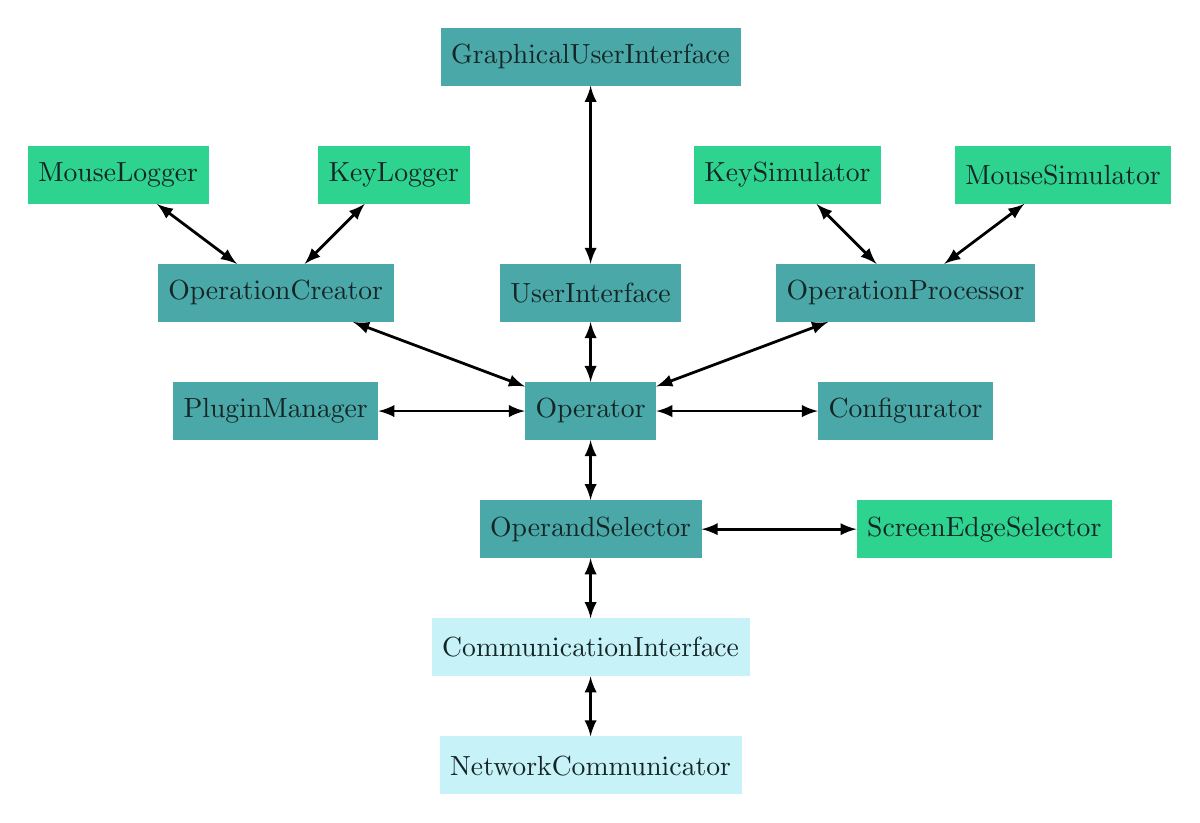
\begin{tikzpicture}
\node[dn] (gui) at (6, 3) {\nodegui};
\node[dn] (ui) at (6, 0) {\nodeui};
\node[dn] (pm) at (2, -1.5) {\nodepm};
\node[dn] (conf) at (10, -1.5) {\nodeconf};
\node[dn] (o) at (6, -1.5) {\nodeo};
\node[dn] (oc) at (2, 0) {\nodeoc};
\node[dn] (op) at (10, 0) {\nodeop};
\node[dn] (os) at (6, -3) {\nodeos};
\node[bn] (ci) at (6, -4.5) {\nodeci};
\node[bn] (nm) at (6, -6) {\nodenm};
\node[gn] (ml) at (0, 1.5) {\nodeml};
\node[gn] (kl) at (3.5, 1.5) {\nodekl};
\node[gn] (ms) at (12, 1.5) {\nodems};
\node[gn] (ks) at (8.5, 1.5) {\nodeks};
\node[gn] (ses) at (11, -3) {\nodeses};
\draw [<->] (gui) -- (ui);
\draw [<->] (ui) -- (o);
\draw [<->] (pm) -- (o);
\draw [<->] (o) -- (conf);
\draw [<->] (oc) -- (o);
\draw [<->] (o) -- (op);
\draw [<->] (kl) -- (oc);
\draw [<->] (ml) -- (oc);
\draw [<->] (op) -- (ks);
\draw [<->] (op) -- (ms);
\draw [<->] (o) -- (os);
\draw [<->] (os) -- (ci);
\draw [<->] (ci) -- (nm);
\draw [<->] (os) -- (ses);
\end{tikzpicture}
\captionof{figure}{Spuštění - načtení operací}
\end{center}

\subsubsection{Připojení k síti}
Nyní začne pracovat CommunicationInterface a NetworkCommunicator, který se buď připojí k existující síti nebo se domluví s ostatními NetworkCommunicatory na vytvoření nové sítě a po jejím vytvoření se k ní připojí (viz sekci "Síť").
\begin{center}
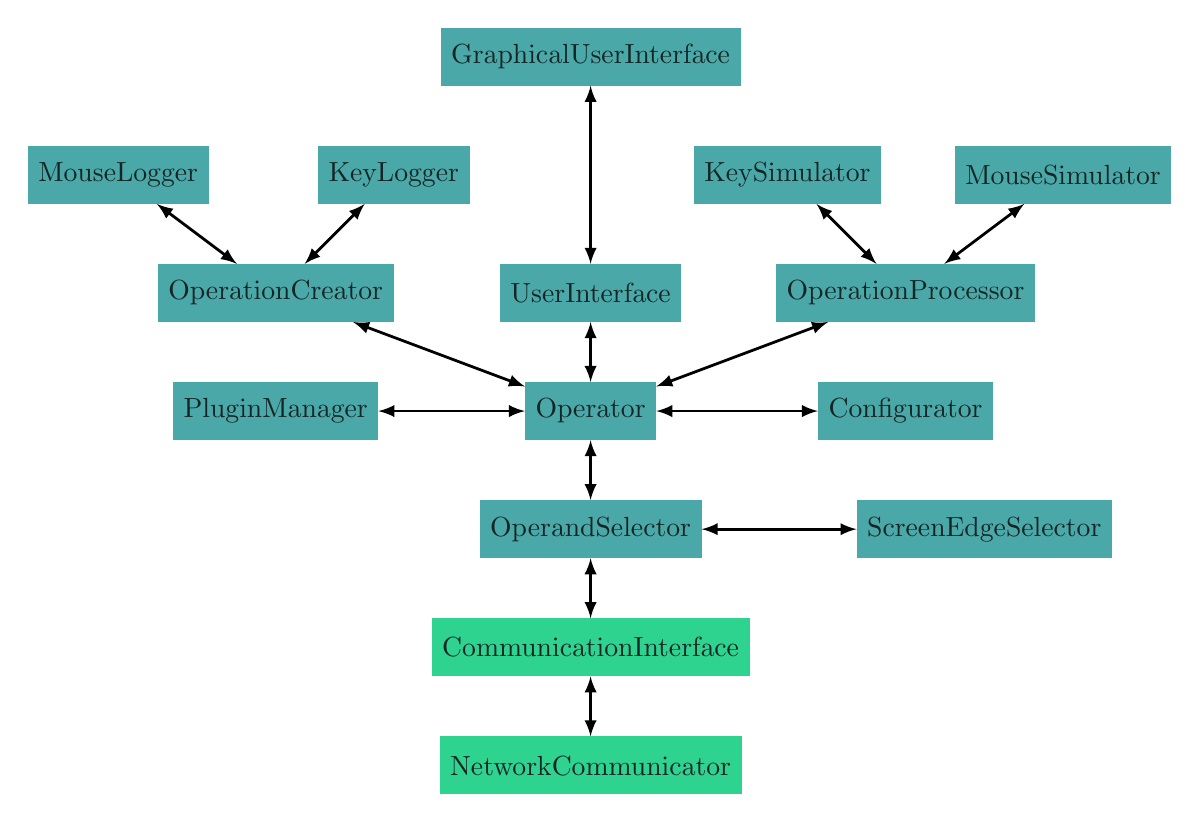
\begin{tikzpicture}
\node[dn] (gui) at (6, 3) {\nodegui};
\node[dn] (ui) at (6, 0) {\nodeui};
\node[dn] (pm) at (2, -1.5) {\nodepm};
\node[dn] (conf) at (10, -1.5) {\nodeconf};
\node[dn] (o) at (6, -1.5) {\nodeo};
\node[dn] (oc) at (2, 0) {\nodeoc};
\node[dn] (op) at (10, 0) {\nodeop};
\node[dn] (os) at (6, -3) {\nodeos};
\node[gn] (ci) at (6, -4.5) {\nodeci};
\node[gn] (nm) at (6, -6) {\nodenm};
\node[dn] (ml) at (0, 1.5) {\nodeml};
\node[dn] (kl) at (3.5, 1.5) {\nodekl};
\node[dn] (ms) at (12, 1.5) {\nodems};
\node[dn] (ks) at (8.5, 1.5) {\nodeks};
\node[dn] (ses) at (11, -3) {\nodeses};
\draw [<->] (gui) -- (ui);
\draw [<->] (ui) -- (o);
\draw [<->] (pm) -- (o);
\draw [<->] (o) -- (conf);
\draw [<->] (oc) -- (o);
\draw [<->] (o) -- (op);
\draw [<->] (kl) -- (oc);
\draw [<->] (ml) -- (oc);
\draw [<->] (op) -- (ks);
\draw [<->] (op) -- (ms);
\draw [<->] (o) -- (os);
\draw [<->] (os) -- (ci);
\draw [<->] (ci) -- (nm);
\draw [<->] (os) -- (ses);
\end{tikzpicture}
\captionof{figure}{Spuštění - připojení k síti}
\end{center}

\subsubsection{Spouštění dokončeno}
Ve chvíli připojení se k síti se v GUI zobrazí ovládací panel a podle instrukcí uživatele se začnou zpracovávat operace.
\begin{center}
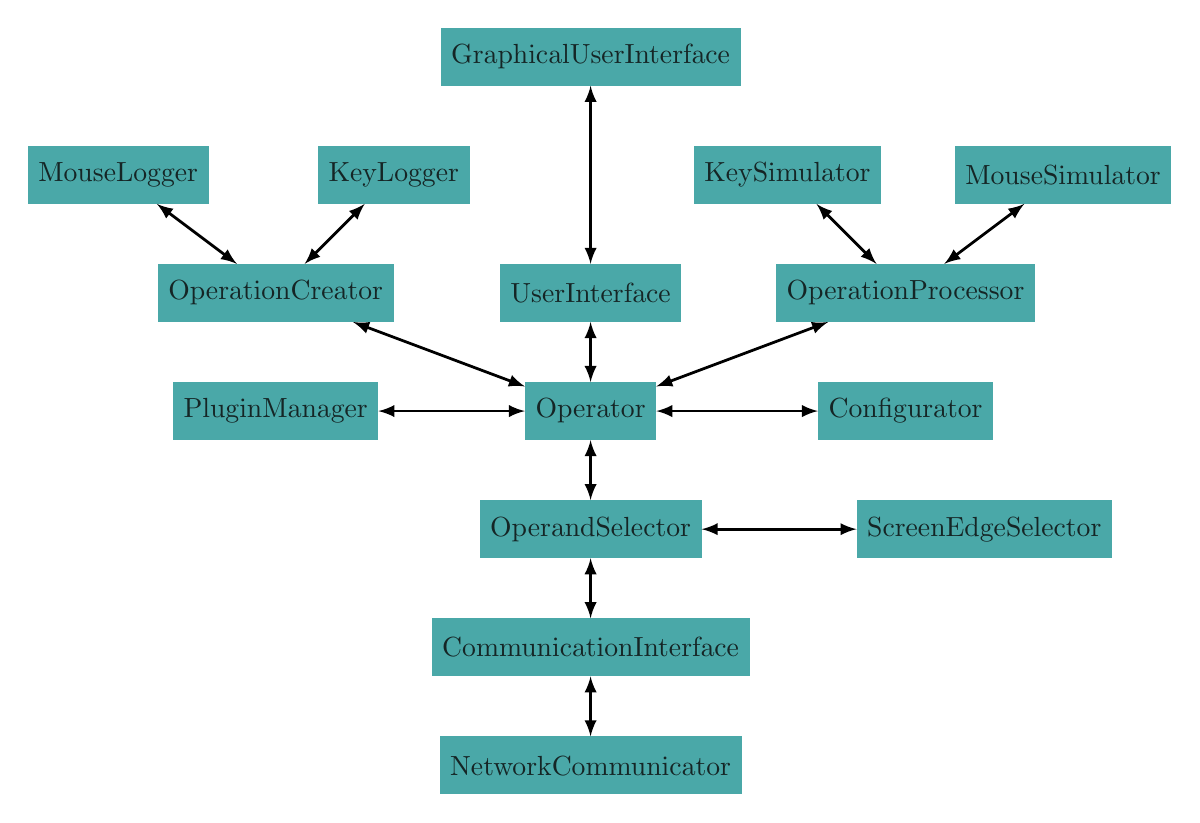
\begin{tikzpicture}
\node[dn] (gui) at (6, 3) {\nodegui};
\node[dn] (ui) at (6, 0) {\nodeui};
\node[dn] (pm) at (2, -1.5) {\nodepm};
\node[dn] (conf) at (10, -1.5) {\nodeconf};
\node[dn] (o) at (6, -1.5) {\nodeo};
\node[dn] (oc) at (2, 0) {\nodeoc};
\node[dn] (op) at (10, 0) {\nodeop};
\node[dn] (os) at (6, -3) {\nodeos};
\node[dn] (ci) at (6, -4.5) {\nodeci};
\node[dn] (nm) at (6, -6) {\nodenm};
\node[dn] (ml) at (0, 1.5) {\nodeml};
\node[dn] (kl) at (3.5, 1.5) {\nodekl};
\node[dn] (ms) at (12, 1.5) {\nodems};
\node[dn] (ks) at (8.5, 1.5) {\nodeks};
\node[dn] (ses) at (11, -3) {\nodeses};
\draw [<->] (gui) -- (ui);
\draw [<->] (ui) -- (o);
\draw [<->] (pm) -- (o);
\draw [<->] (o) -- (conf);
\draw [<->] (oc) -- (o);
\draw [<->] (o) -- (op);
\draw [<->] (kl) -- (oc);
\draw [<->] (ml) -- (oc);
\draw [<->] (op) -- (ks);
\draw [<->] (op) -- (ms);
\draw [<->] (o) -- (os);
\draw [<->] (os) -- (ci);
\draw [<->] (ci) -- (nm);
\draw [<->] (os) -- (ses);
\end{tikzpicture}
\captionof{figure}{Spuštění - dokončeno}
\end{center}

\subsection{Proces ukončení}
Ve chvíli, kdy uživatel ukončí program, zmizí GUI, pozastaví se probíhající operace, NetworkCommunicator se odpojí od sítě a ukončí se všechna vlákna, čímž se ukončí i vlastní program. Uživatel z ukončení NetworkOperatoru bude mít pocit, že je "hned" hotové.

\subsection{Cílová platforma}
Program bude naprogramován převážně v C\#u, avšak k zajištění fungování některých jeho funkcí bude potřebovat používat Windows API, k němuž bude přistupovat pomocí knihoven napsaných v C++ (které budu za tímto účelem vytvářet spolu se zápočtovým programem), což způsobí závislost programu na operačním systému Windows. Druhý důvod, proč bude NetworkOperator kompatibilní pouze s Windows, je použití WPF k naprogramování GUI.\\\\
Testování bude prováděno na počítači s Windows 7 a Windows 10, oboje aktualizované na současnou verzi, kompatibilita s jinými verzemi Windows zvláštním způsobem ověřována nebude, ovšem program bude napsán tak, aby pracoval na všech Microsoftem podporovaných desktopových verzích Windows. Ale testování programu například na Windows 8 prováděno nebude.

\newpage
\section{Plán splnění požadavků jednotlivých předmětů}
V následujícím seznamu je ke každému předmětu uvedeno, co za technologii probíranou na přednáškách k danému předmětu primárně plánuji netriviálně použít ve svém zápočtovém programu:
\begin{enumerate}[leftmargin=5mm]
\item NPRG035 (C\# - zima) - bez specifikace
\item NPRG038 (.NET I) - síťování, reflection, vláknování
\item NPRG057 (.NET II) - spolupráce C\#u a C++
\item NPRG064 (.NET UI) - WPF
\end{enumerate}
Co se týče minimální velikosti zdrojových kódů, tu, věřím, dodržím.

\end{document}
